
\section{mass continuity}

\begin{frame}{the most basic shallow assumption}

\begin{columns}

\begin{column}{0.6\textwidth}
\begin{itemize}
\item there are many shallow theories: SIA, SSA, hybrids, Blatter, \dots
\item \emph{all} make one assumption not required in the (non-shallow) Stokes theory:

\begin{center}
\emph{the surface and base of the ice are given by differentiable functions} $z=h(t,x,y)$ \emph{and} $z=b(t,x,y)$
\end{center}
\item surface overhang is not allowed
\end{itemize}
\end{column}

\begin{column}{0.4\textwidth}
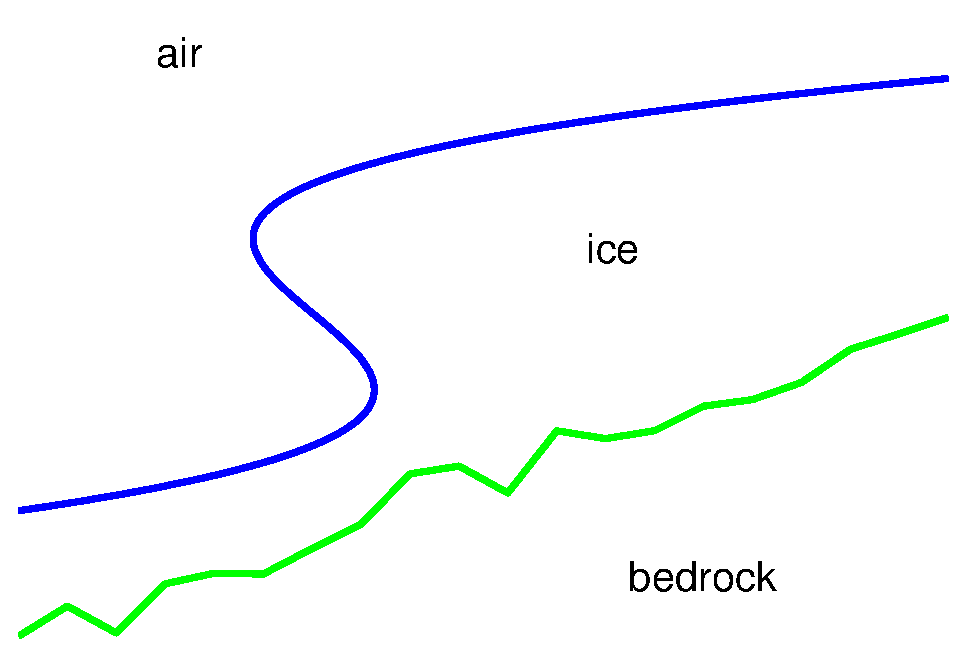
\includegraphics[width=1.0\textwidth]{sshape}

\scriptsize
\begin{center}
\alert{not shallow!}
\end{center}
\vspace{6mm}

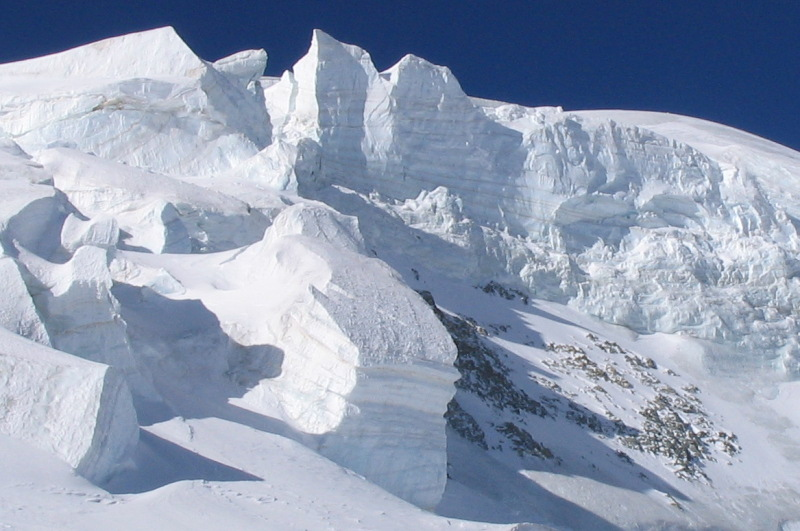
\includegraphics[width=1.0\textwidth]{Serac2}

\begin{center}
\alert{not shallow!}
\end{center}
\end{column}
\end{columns}
\end{frame}


\begin{frame}{kinematic and mass continuity equations}

\begin{itemize}
\item what does this ``most basic shallow assumption'' get you?
\item \emph{answer:} a map-plane mass continuity equation
\item consider these three equations:
  \begin{itemize}
  \item[$\circ$]  the surface kinematical equation
  \item[$\circ$]  the base kinematical equation
  \item[$\circ$]  the map-plane mass continuity equation
  \end{itemize}
\item under the ``most basic shallow assumption'', 

\begin{center}\emph{any two imply the third}\end{center}

\vspace{5mm}
\item these three equations are on the next slide
\end{itemize}
\end{frame}


\begin{frame}{kinematic and mass continuity equations 2}

\begin{itemize}
\item $a$ is surface mass balance ($a>0$ is accumulation)
\item $s$ is basal melt rate ($s>0$ is basal melting)
\item $M=a-s$
\item define the map-plane flux of ice,
	$$\bq = \int_{b}^{h} (u,v)\,dz = \overline{\mathbf{U}}\,H$$
\item the three equations are:
\begin{empheq}[left=\text{surface kinematical}\quad,innerbox=\fbox]{equation}
h_t = a - u\big|_h h_x - v\big|_h h_y + w\big|_h  \label{surfkine}
\end{empheq}
\begin{empheq}[left=\text{base kinematical}\quad,innerbox=\fbox]{equation}
b_t = s - u\big|_b b_x - v\big|_b b_y + w\big|_b  \label{basekine}
\end{empheq}
\begin{empheq}[left=\text{mass continuity}\qquad\qquad\qquad\quad,innerbox=\fbox]{equation}
H_t = M - \Div \bq \label{masscontinuity}
\end{empheq}
\end{itemize}
\end{frame}


\begin{frame}{kinematic and mass continuity equations 3}

\begin{itemize}
\small
\item how are the three equations related to each other?
\item start with the incompressibility of ice
    $$u_x + v_y + w_z = 0 \qquad \iff \qquad w_z = - \Div \mathbf{U}$$
\item integrate vertically:
    $$w\big|_h - w\big|_b = \int_b^h w_z\,dz = - \int_b^h \Div \mathbf{U}\,dz$$
\item now be careful and use the Leibniz rule for differentiating integrals:
\scriptsize
  \begin{align*}
\frac{d}{dx}\left(\int_{A(x)}^{B(x)} F(x,y)\,dy\right) &= B'(x) F(x,B(x)) - A'(x) F(x,A(x)) + \int_{A(x)}^{B(x)} F_x(x,y)\,dy
  \end{align*}
\small
\item which implies that
   $$- \Div \int_b^h \mathbf{U}\,dz = - \grad h \cdot \mathbf{U}\big|h + \grad b \cdot \mathbf{U}\big|_b - \int_b^h \Div \mathbf{U}\,dz$$
\item so
    $$w\big|_h - w\big|_b = - \Div \mathbf{q} + \grad h \cdot \mathbf{U}\big|h - \grad b \cdot \mathbf{U}\big|_b$$
\item and so on
\normalsize
\end{itemize}
\end{frame}


\begin{frame}{kinematic and mass continuity equations 4}

\begin{itemize}
\item why am I telling you this?
\item because glaciology articles are filled with recapitulation of these equivalences

\vspace{5mm}
\item my main points regarding mass continuity:
  \begin{itemize}
  \item[$\circ$] most ice sheet models use the mass continuity equation to describe change in ice sheet geometry
  \item[$\circ$] but they could instead use the surface kinematical equation
  \item[$\circ$] and they almost always use, and greatly simplify, the basal kinematical equation
  \end{itemize}
\end{itemize}
\end{frame}


\begin{frame}{standard recipe for ice sheet models}

\begin{itemize}
\item the ingredients of a typical ice sheet model:
  \begin{enumerate}
  \item numerical implementation of a stress balance: gives velocity $\mathbf{u}=(u,v,w)$
  \item from the horizontal velocity $\mathbf{U}=(u,v)$, or the horizontal flux $\mathbf{q}$, and the climatic mass (surface) balance $M$, do a time-step of the mass continuity equation to get $\Delta H = H_t \Delta t$
  \item update upper (and perhaps lower) surface elevation: $h \mapsto h+H_t \Delta t$
  \item decide on next time-step $\Delta t$, and repeat at 1.
  \end{enumerate}

\vspace{5mm}
\item the non-sliding SIA is slightly atypical because we can write $\mathbf{q} = - D \grad h$ in addition to $\mathbf{q} = \overline{\mathbf{U}}H$
\end{itemize}
\end{frame}
